\section{Conclusions}

In this paper, we present the stories behind the development of EnsembleDashVis, an interactive dashboard designed to visualize the input parameters and outcomes of an \ac{ABC-SMC} inference model used to analyze COVID-19 data collected during the first wave of the outbreak in Scotland.

Given the multitude of uncertainties and challenges during this exceptional period, a considerable amount of information was unavailable to us during the development process. It was only through the Scottish COVID-19 Response Consortium Stakeholder Report \cite{abdalla2021Scottish}, published in late 2021, and various publications \cite{chen2022RAMPVIS,dykes2022Visualizationb,khan2022Propagating,khan2022Rapid,rydow2023RAMPVIS} that unveiled the remarkable endeavors undertaken by other volunteer teams, that we gained additional insight and details.

\begin{figure}[tb!]
    \centering
    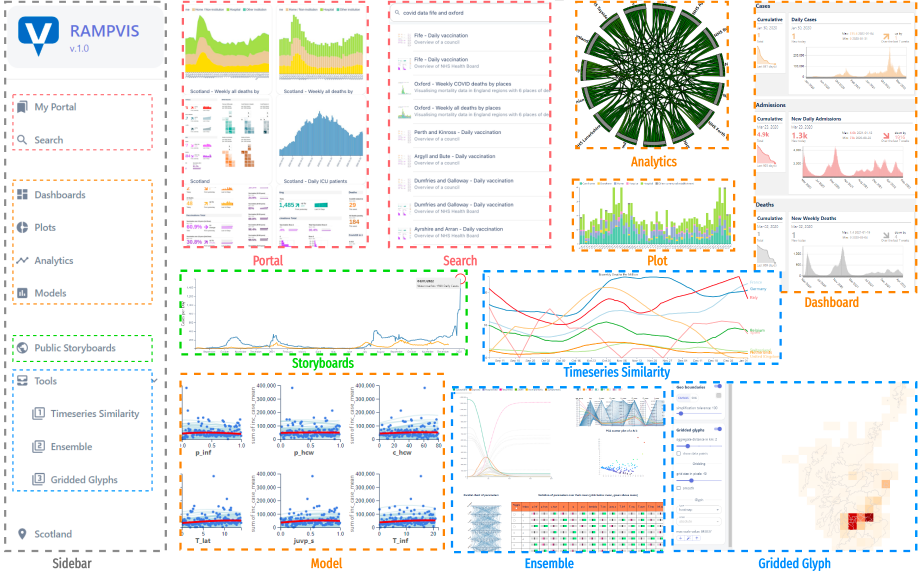
\includegraphics[width=\linewidth]{rampvis.png}
    \caption{EnsembleDashVis has undergone extensive development by multiple UK institutions and is currently maintained by the Oxford e-Research Centre at the University of Oxford, serving as a vital element of the RAMPVIS infrastructure. It is well-prepared to offer rapid and invaluable visualization support for future emergency responses. Image courtesy of Rydow et al. \cite{rydow2023RAMPVIS}.
    }
    \label{fig:rampvis}

\end{figure}

We hope that our experience serves as a valuable source of insight on how VIS research and techniques can play a crucial role in emergency response initiatives and aid in effectively preparing for future emergencies.